\chapter{Class diagram}
\section{Common Layer}
The class diagram shown in figure \ref{fig:commonoverview} gives an overview of all the classes (but doesn't show all the relations!). This overview is to clarify that the \emph{FlowNetworkEntity} have a \texttt{"has-a"} relationship with the components (\emph{MergerEntity, PumpEntity...}).

In figure \ref{fig:classcomponents} the class diagram gives a more detailed view of the components and in more detail how the pipes are connected. Very noticeable are the interfaces \emph{IFlowOutput} and \emph{IFlowInput}. Since a component can have more than 1 input/output an array is used, whereby the pipe also needs to understand to which output it is connected hence the pipe also has the index pipe.

\section{Presentation Layer}
TODO

\section{Business Layer}
TODO

\section{Data Access layer}
Figure \ref{fig:dataaccess} shows the class diagram of the Data Access layer, the Data Access Layer is small and it could be considered to move this to the business layer. When you open a file you get a dumb model back (objects from common) because otherwise the system is failing to follow Separation of Concerns in SOLID principals.

\begin{figure}[h!]
	\centering
	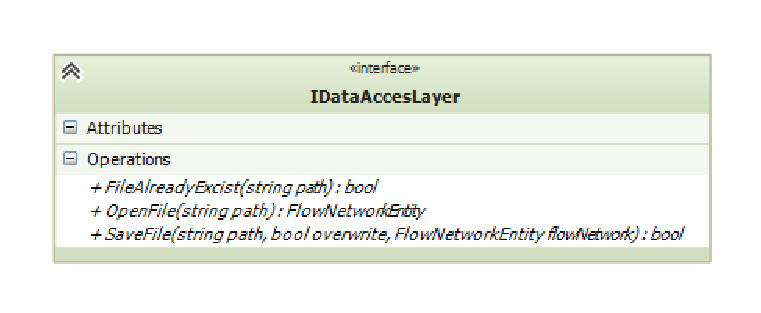
\includegraphics{figures/ClassDataAccess.pdf}
	\caption{Class Diagram Data Access Layer}
	\label{fig:dataaccess}
\end{figure}

\begin{sidewaysfigure}[h!]
	\centering
	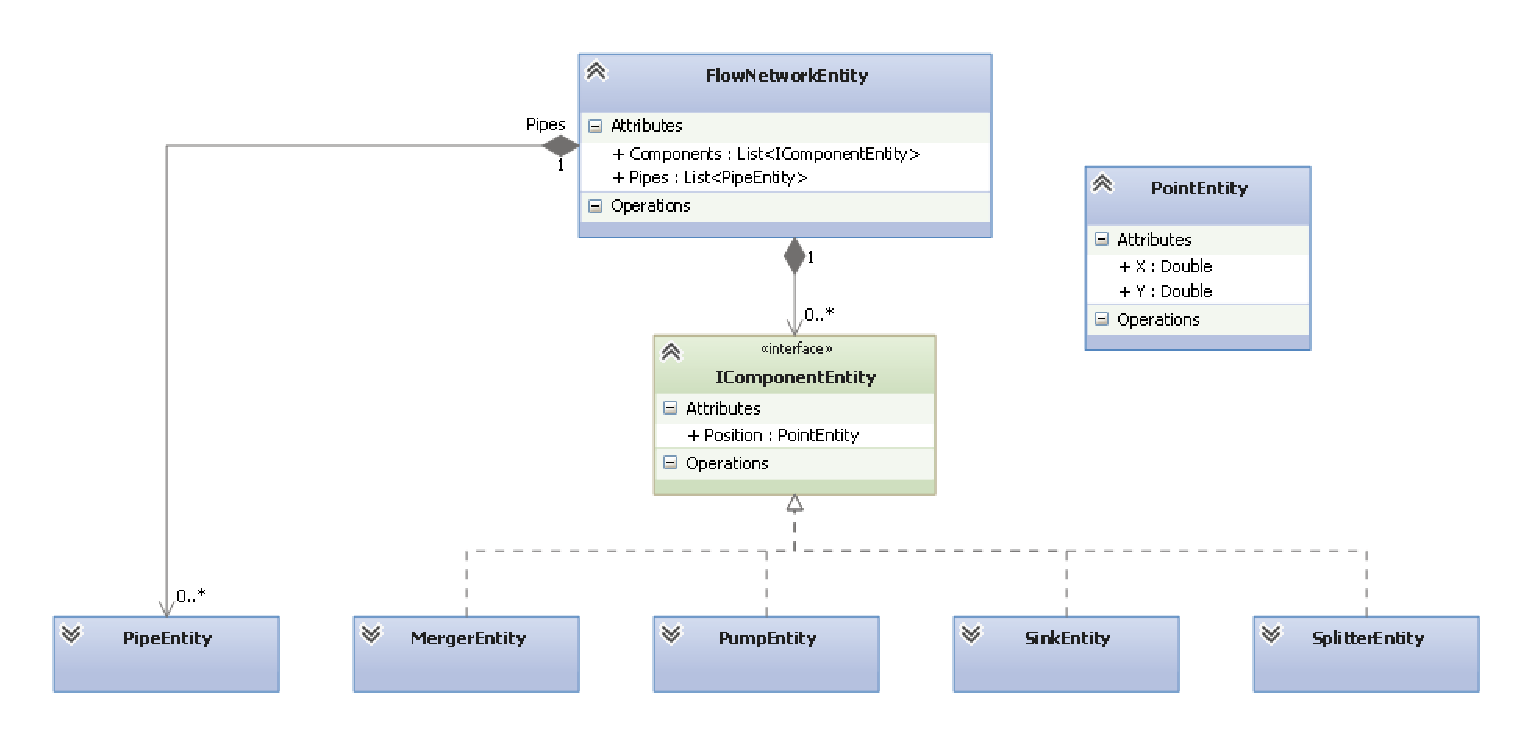
\includegraphics[width=\textwidth]{figures/ClassCommonOverall.pdf}
	\caption{Class Diagram Common overview}
	\label{fig:commonoverview}
\end{sidewaysfigure}

\begin{sidewaysfigure}[h!]
	\centering
	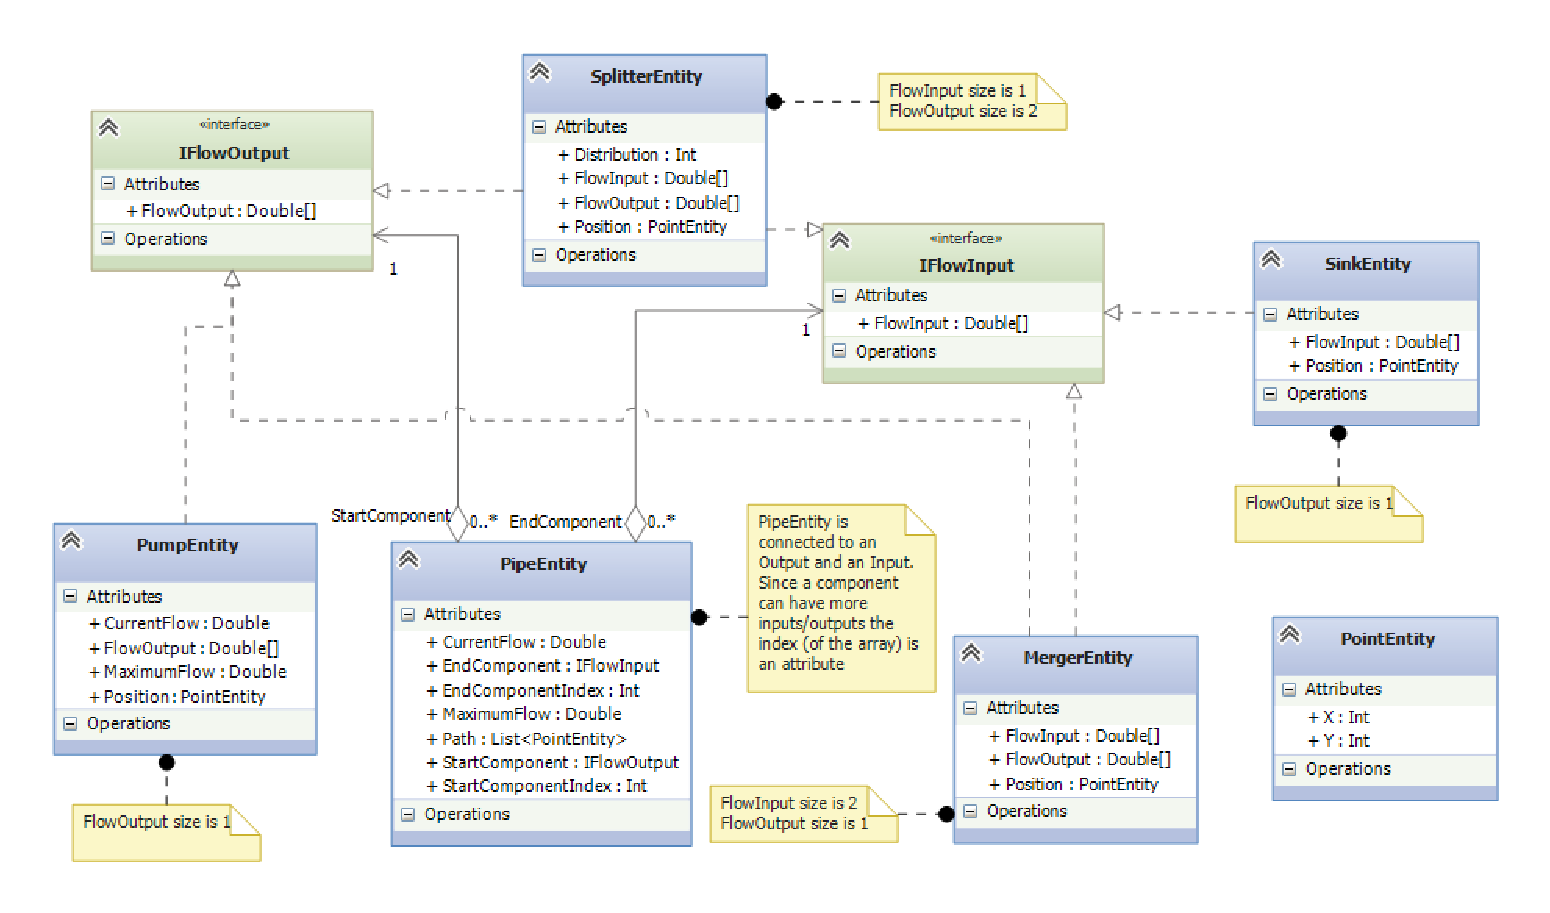
\includegraphics[width=\textwidth]{figures/ClassCommonComponents.pdf}
	\caption{Class Diagram Common Components}
	\label{fig:classcomponents}
\end{sidewaysfigure}